\chapter{Spawning and catching}
Pokémon GO is intended to be played on the move

\label{chap:spawn}
\textbf{FIXME}

\section{Wild spawns}
\label{sec:spawns}
\textbf{FIXME}

\subsection{Lures and incense}
Spawn rates can be increased by means of Incense and Lures.
Incense lasts for an hour, affects only the Trainer using it (i.e.\ other Trainers
  will neither see nor be able to interact with resulting spawns),
  and moves with the Trainer.
A Trainer can make use of only one incense at a time\footnote{The
  ``Mystery Box'', Sunsteel Strike Adventure Effect, and
  Moongeist Beam Adventure Effect similarly cannot be used
  alongside incense, or each other.}.
Incense will result in a spawn every five minutes for immobile Trainers.
Otherwise, incense will result in a spawn every 200 meters moved.
Incense is awarded at certain Trainer levels and for some Research,
  and can be bought for 40 Pokécoins (or eight for 250).
Additionally, once unlocked, the Trainer can use Adventure Incense.
This special incense results in a greater diversity of spawns.
So long as it is completely used by midnight, it is automatically replenished
  upon the change of day.
Adventure incense lasts fifteen minutes, so using it after 2344h will suppress
  the next day's portion.
There is a small chance of spawning the Legendary ``Galarian birds'' while
  using Adventure incense.
\textbf{FIXME}
\begin{figure}[h!]
  \begin{minipage}[t]{0.5\textwidth}
    \begin{center}
    
\includegraphics[scale=.4]{images/incense.png}
    \end{center}
    \caption*{Incense}
    \label{fig:incense}
  \end{minipage}
  \begin{minipage}[t]{0.5\textwidth}
    \begin{center}
    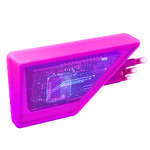
\includegraphics[scale=.4]{images/lure.png}
    \end{center}
    \caption*{Lure module}
    \label{fig:lure}
  \end{minipage}
\end{figure}

\section{Catching}
\label{sec:catch}
\textbf{FIXME}

\subsection{Berries}
\begin{figure}[h!]
  \begin{minipage}[t]{0.3\textwidth}
    \begin{center}
    
\includegraphics[scale=.4]{images/razz.png}
    \end{center}
    \caption*{Razz berry}
    \label{fig:razz}
  \end{minipage}
  \begin{minipage}[t]{0.3\textwidth}
    \begin{center}
    
\includegraphics[scale=.4]{images/nanab.png}
    \end{center}
    \caption*{Nanab berry}
    \label{fig:nanab}
  \end{minipage}
  \begin{minipage}[t]{0.3\textwidth}
    \begin{center}
    
\includegraphics[scale=.4]{images/pinap.png}
    \end{center}
    \caption*{Pinap berry}
    \label{fig:pinap}
  \end{minipage}
\end{figure}
Berries can enhance the catching process (\autoref{table:berries}).
Only one Berry can be applied to a Pokémon at a time.
If a Berry is active, its icon will be shown on the encounter summary.
The Berry is consumed upon use, but persists on the Pokémon across Pokéballs
  and even encounters (i.e., you can leave the encounter, and if you return,
  the Berry will still be applied).
If the Pokémon escapes a Pokéball, however, any applied Berry is gone forever.
A new Berry can be used in this case.
\begin{table}[ht]
\begin{center}
  \begin{tabular}{lp{.75\textwidth}}
Berry & Effect \\
\Midrule
Razz  & 150\% catch percentage\\
Nanab & Immobilizes Pokémon\\
Pinap & Boosts Candy rewards: 3→7, 5→11, 10→23\\
Silver pinap & 180\% catch percentage\newline Boosts Candy rewards: 3→7, 5→11, 10→23\\
Golden razz & 250\% catch percentage\newline Restore full HP to Gym defender\\
\end{tabular}
\end{center}
\caption{Berries and their uses}
\label{table:berries}
\end{table}
\begin{figure}[h!]
  \begin{minipage}[t]{0.5\textwidth}
    \begin{center}
    
\includegraphics[scale=.4]{images/silverpinap.png}
    \end{center}
    \caption*{Silver pinap berry}
    \label{fig:silverpinap}
  \end{minipage}
  \begin{minipage}[t]{0.5\textwidth}
    \begin{center}
    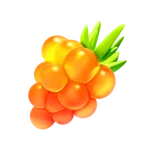
\includegraphics[scale=.4]{images/goldenrazz.png}
    \end{center}
    \caption*{Golden razz berry}
    \label{fig:goldenrazz}
  \end{minipage}
\end{figure}

\section{Shiny Pokémon and other visual forms}
\label{sec:shiny}
Many Pokémon have an alternate presentation known as their ``Shiny'' form.
These forms are collected in their own Pokédex (\autoref{sec:dexen}).
Shadow and Purified Pokémon can be Shiny.
Shininess is preserved across evolution, purification, and trades.
Shininess is not determined at the scope of Pokémon spawns, but for individual
  Trainers' encounters: two Trainers encountering the same spawn might disagree
  on whether or not it is Shiny.
Shiny forms are fairly rare (\autoref{table:shiny}), but various events
  enhance the probability of their generation.
\begin{table}[ht]
\begin{center}
\begin{tabular}{ll}
Context & Probability of shine \\
\Midrule
  Wild spawns & 1/512 (0.195\%) \\
  Team GO Rocket Grunt shadows & 1/256 (0.39\%) \\
  Team GO Rocket Leader shadows & 1/64 (1.56\%) \\
  5🟉 raid & 1/20 (5\%) \\
\end{tabular}
\end{center}
\caption{Likelihood of Shiny Pokémon}
\label{table:shiny}
\end{table}

Despite offering no advantage in battle, and being in no way associated with
  higher levels or IVs, Shiny forms are of great importance to many players.
Personally, unless I expect to trade them, I transfer them to the Professor
  without a second thought.
His usual culinary magic leads to a particularly shiny feast of harvested Pokésoul.

Events sometimes make possible special backgrounds or clothed forms.
Froufrou's uselessness in combat is matched only by its
  capacity for wasting Stardust taking on any number of visual forms.
I don't intend to get into the topic any further.
